\chapter{Background}
\label{ch:background}
This chapter introduces some background material that serves as the basis for this thesis, covering in part the various topics it touches. The chapter is meant only to introduce these topics, and provide brief summarizations. Some additional background material, more specifically \emph{related work}, is covered in Ch.~\ref{ch:related_work}. 

\section{Software Modeling and Modeling Languages}
\label{sec:software_modeling}
In the world of software development, potential problems and challenges that may arise when developing a product are plentiful. In anything but trivial systems, bugs are almost inevitable, and may be caused by anything from plain programming errors to intermittent problems as a result of resource contention. Systems with concurrent behavior are particularly difficult to implement sensibly, as there are several additional complexities and pitfalls associated with these. Potential problems are also not only related to bugs, but possibly also performance and correctness.

\noindent
In addition to many types of software being nontrivial to implement, keeping the code \emph{readable} is an undertaking of its own. When new developers are added to a team that is already deep into the development process, it can take significant time and effort to become familiar with the system. This can be a result of several factors, such as different code styles, massive spread of code (over a vast amount of files or classes), or simply bad code. In many cases, we may also want non-programmers, such as customers or salespeople, to understand what the system does.

\noindent
Software modeling serves as a solution for smoothing out these processes. Instead of the system specification existing only as code a list of functionality and bugs, it is possible to create a visual and formal model of the system. Such models are more readily understood by non-programmers, and also help other developers become familiar with the overall system architecture more quickly.

\subsection{The Purpose of Software Modeling}
\label{sec:software_modeling_purpose}
The real world is often complex, and correctly expressing this complex world in terms a computer can understand is not a trivial task. Software modeling in languages such as the \gls{uml} or the \gls{sdl} is a useful tool, helping smooth out this process in several ways.

\paragraph{Conceptual Abstractions} The most important purpose of software models is perhaps to provide \emph{conceptual abstractions}, by describing system functionality and collaborations on a higher level, removing less relevant detail~\cite{braek:itut_methodologies}. This allows developers and other interested parties to get a clear overview of the system architecture, without having to dig through thousands of lines of code.

\paragraph{Understandability} In addition to providing abstractions that hide details, software models are able to present architecture and functional concepts in ways that better appeal to our intuition~\cite{selic:model_driven_development}. This further reduces the learning effort required, and may help us to a better understanding of the workings of a system.

\paragraph{Separation of Concerns} Another purpose of software modeling is \emph{separation of concerns}, which involves reducing the perceived complexity of the system by modeling parts that are fairly independent as separate, but collaborating, entities~\cite{braek:itut_methodologies}. This may also allow the system to be modularized, potentially simplifying both implementation and maintenance of the system.

\paragraph{Formal Analysis} With the use of formal and well-established modeling methods, we also open up the system design to formal analysis. Depending on the method, we may be able to mathematically or logically analyze the system architecture in order to uncover inconsistencies or errors, or calculate additional system requirements such as hardware capabilities or bandwidth. This also adds \emph{predictiveness} to the system, providing indications of how the final implementation will behave under various conditions~\cite{selic:model_driven_development}.

\subsection{UML Activities}
\label{sec:uml_activities}
The \gls{uml} Activity diagram is a modeling concept suitable for expressing processes and workflows, particularly where concurrent behavior is observed. \gls{uml} Activities use \emph{Petri-net-like} semantics, and can be mathematically or logically verified in various ways~\cite{eshuis:uml_verification, kraemer:arctis, storrle:uml_verification}.

\noindent
In general, \gls{uml} Activity diagrams may consist of a number of different types of elements. These include, among others, logical elements such as \emph{forks} and \emph{joins}, allowing concurrent execution and synchronization of these. Other examples are \emph{decisions}, implementing alternate branches, and \emph{wait nodes}, allowing the application to wait for an event before continuing execution.  The activity is executed as a series of \emph{activity steps}, where each step involves performing the logic of one or more elements. An example of a \gls{uml} Activity diagram containing many of these elements is displayed in Fig.~\ref{fig:activity_diagram}. The various elements are described in more detail within the context of Reactive Blocks, in Sect.~\ref{sec:reactive_blocks}.

\begin{figure}[htp]
	\centering
	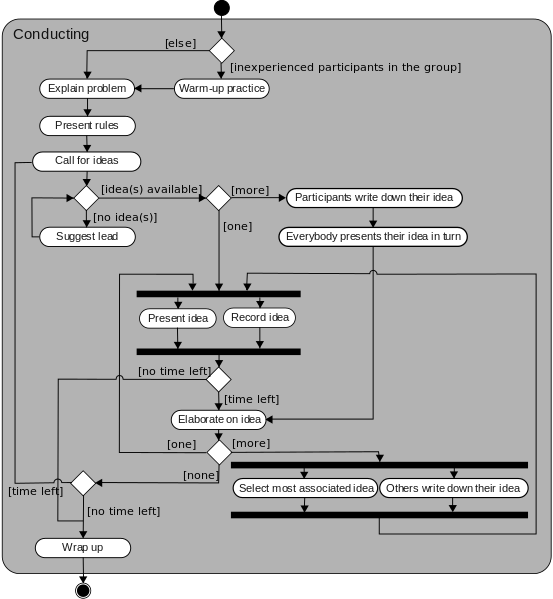
\includegraphics[width=0.8\textwidth]{activity_diagram}
	\caption[UML Activity Diagram]{An UML Activity diagram for a brainstorming process. The process consists of various \emph{actions}, such as ``Explain problem'' or ``Present idea'', that are separated primarily by conditional logic through \emph{decisions}. We also see some examples of concurrent behavior with synchronization, more specifically before and after the ``Present idea'' and ``Record idea'' actions. Both actions are performed simultaneously, and execution does not continue until both actions have finished. We also see the start and end points of activity execution, the \emph{initial node} and the \emph{final node}, as the two black circles above and below the gray area. \emph{Image source: \url{http://en.wikipedia.org/wiki/Activity_diagram}}}
	\label{fig:activity_diagram}
\end{figure}

\subsection{Model-Driven Development}
\label{sec:model_driven_development}
While software modeling simply can be used to provide better documentation of systems and visualize their architecture, it is also possible to go one step further and employ the \emph{\gls{mdd}} approach (closely related to the concept of \emph{\gls{mda}}\footnote{\href{http://www.omg.org/mda/}{OMG: MDA - The Architecture Of Choice For A Changing World (link)}}). With the \gls{mdd} approach, software models are at the center of the development process, rather than playing a supplementing or secondary role. Software models have the advantage that they can be very independent from the implementation platforms, allowing the software structure to be mapped, or \emph{deployed}, to more than one platform~\cite{braek:itut_methodologies, selic:model_driven_development}.

\noindent
Digging deeper into the \gls{mdd} approach, it has been argued that its full potential can only be realized if the models are used to automatically generate complete and fully executable programs~\cite{selic:model_driven_development}. Given a robust and correct deployment, automatic generation of code can help improve correctness, maintainability, and number of software bugs.

\noindent
There are various commercial and non-commercial projects working on solutions for \gls{mda} and \gls{mdd}, many of them listed on the \gls{omg} website.\footnote{\href{http://www.omg.org/mda/committed-products.htm}{OMG: MDA - Committed Companies And Their Products (link)}} Reactive Blocks, currently in development by Bitreactive AS,\footnote{\href{http://www.bitreactive.com/}{Bitreactive website (link)}} is an example of a solution that generates fully executable applications based on \gls{uml} Activity-like models.

\subsection{Reactive Blocks}
\label{sec:reactive_blocks}
Reactive Blocks is the result of various research efforts in the field of compositional service engineering and \gls{mdd} at \gls{ntnu}\cite{kraemer:arctis_ramses}. The software is released as a plugin for the Eclipse IDE, providing a modeling environment for \gls{uml} Activities. Using the Reactive Blocks tool, these models can be formally analyzed, and further used to automatically generate fully executable applications.

\noindent
Models Reactive Blocks are based on and very closely resemble \gls{uml} Activity diagrams. Figure~\ref{fig:reactive_blocks_model} shows an example of a model in Reactive Blocks, containing many of the \gls{uml} Activity elements mentioned in Sect.~\ref{sec:uml_activities}. Reactive Blocks is additionally focused around \emph{Collaborative Building Blocks}, allowing complete collaborations or sub-services to be reused in the form of building blocks.

\begin{figure}[htp]
	\centering
	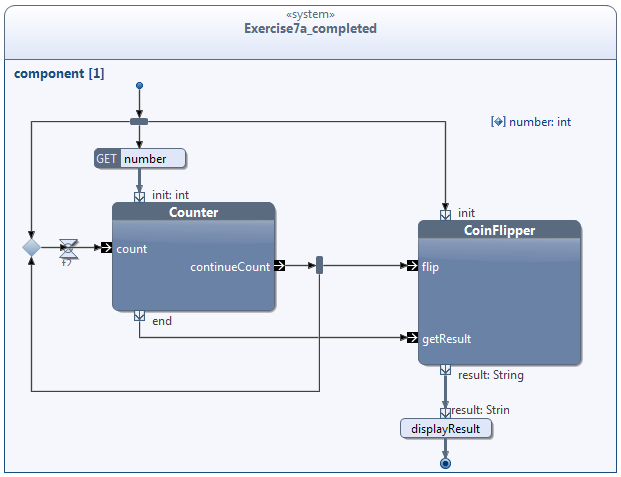
\includegraphics[width=1\textwidth]{reactive_blocks_model}
	\caption[Reactive Blocks model example]{An example of a model in Reactive Blocks, resembling the \gls{uml} Activity diagram in Fig.~\ref{fig:activity_diagram}. The \emph{Counter} and \emph{CoinFlipper} elements are building blocks, containing modularized logic exposed through an \gls{api}.}
	\label{fig:reactive_blocks_model}
\end{figure}

\noindent
Activities in Reactive Blocks are executed like regular \gls{uml} Activities, as a series of \emph{activity steps}. These steps are implemented in the form of \emph{tokens} moving through sequences of elements (\emph{flows}), activating them along the way. The step finally ends when the token reaches a \emph{stable position}, where it will either stay until the start of another step or be removed. Reactive Blocks models can be built from a number of modeling elements and nodes:

\begin{itemize}
	\item{\textbf{Edge:}} \emph{Edges} connect other elements in Reactive Blocks, carrying tokens and implementing the flow between them. All edges are directed, and may additionally carry data objects with tokens. With data, the edge is called an \emph{object flow}, and without data, simply a \emph{control flow}.
	\item{\textbf{Initial Node:}} The \emph{Initial Node} is where the activity execution starts. When the application is launched, a token is sent out from all initial nodes.
	\item{\textbf{Operation/Java method:}} Corresponding to the \emph{actions} displayed in Fig.~\ref{fig:activity_diagram}, \emph{operations} are elements that work on data or \glspl{api}, implemented in Reactive Blocks as Java methods. Operations may take one or more parameters, and in the case of more, they also work like \emph{join} nodes.
	\item{\textbf{Variables}} \emph{Variables} are elements that store data, and can be accessed by regular operations, or directly within the activity diagram via special \emph{set} and \emph{get} operations.
	\item{\textbf{Flow Final:}} The \emph{Flow Final} node terminates a flow, removing any incoming token.
	\item{\textbf{Activity Final:}} The \emph{Activity Final} node works like the flow final, except it also terminates the application.
	\item{\textbf{Timer:}} The \emph{Timer} node realizes simple delays by putting any incoming tokens in a stable position until the timer has expired, upon when a new activity step is started.
	\item{\textbf{Decision:}} \emph{Decision} nodes are used to implement alternate branches. Incoming tokens must carry data, and the outgoing edge is chosen by checking the carried data against the \emph{guards} set on these edges. Guards may be either boolean, integer or String values, or \emph{null}.
	\item{\textbf{Fork:}} \emph{Fork} nodes are used to implement concurrent branches and parallel behavior, duplicating any incoming tokens to all outgoing edges.
	\item{\textbf{Join:}} The complementary part to forks, the \emph{Join} node synchronizes several flows, concurrent or not. When a token has been received on \emph{all} incoming edges, a \emph{single} token is sent on the outgoing edge.
	\item{\textbf{Merge:}} \emph{Merge} nodes are similar to join nodes, but instead of waiting for a token to arrive on each incoming edge, \emph{all} tokens from incoming edges are simply forwarded on the outgoing edge.
	\item{\textbf{Event Reception:}} \emph{Event Receptions} are stable positions that wait for an internal signal, or an \emph{event}, before sending a token on the outgoing edge. These events are generally sent from operations somewhere else in the system.
	\item{\textbf{Building Blocks:}} \emph{Building Blocks} are independent sub-modules that implement some functionality. These modules are themselves constructed like activity diagrams, but do not have initial or activity final nodes. Instead, they have input/output pins that accept tokens, and \glspl{esm} that determine which pins can accept tokens in a given state. 
\end{itemize}

\noindent
Because it is a tool for \gls{uml} Activity modeling, with model checking and code generation capabilities, Reactive Blocks will serve as the basis for the work in this thesis.

\section{Learning Programming and Software Modeling}
\label{sec:learning_programming}
In order to teach potential users to best utilize topics such as a programming language, programming paradigm, protocol or modeling language, various tools or sources of information may be provided. Generally, some form of formal documentation or specification of the language or protocol is considered mandatory, and serves as the \emph{definitive} source of information.

\noindent
While a topic's documentation often serves as its primary source of information, such formal documents are not necessarily the best source of information when \emph{learning} about the given topic. Often it is not intended as a learning resource, but rather as a formal reference for users already familiar with the topic. In the documentation, the topic is generally presented in a structured way with respect to its various aspects, so that it is easy for someone already familiar with the topic to find the required information.

\noindent
A good example of this is the \gls{uml} specification.\footnote{\href{http://www.omg.org/spec/UML/2.4.1/}{OMG: Documents Associated With Unified Modeling Language (UML), V2.4.1 (link)}} While the specification offers detailed information about every aspect of \gls{uml} in a way that suits an experienced user, it is likely confusing and not particularly helpful for a user with no previous experience or knowledge about \gls{uml}. Using this specification as a starting point for learning \gls{uml} is likely to require a lot of effort from the user. In the worst case, the user may not even learn all the concepts properly, despite the provided information being very specific and accurate.

\noindent
More importantly, the user may not learn how to properly apply the learned concepts to a given situation. There might be subtleties that are difficult to discover without proper guidance, and possibly even potential for misconceptions. This can leave many users with insufficient knowledge and skills within the topic, decreasing the effectiveness and quality of their work, and in the worst case, even preventing them from completing more advanced task.

\noindent
While documentation for a topic undoubtedly is a valuable resource, we can safely conclude that it is not always the best learning tool. It has some advantages, such as generally providing very complete and precise information, but this may simply be too much for novice users to comprehend. Instead, novice users more often turn to \emph{tutorials} when wanting to learn about a new topic. For many topics, various tutorials and exercises are often created in order to provide a better introduction to these, decreasing the threshold for learning.

\section{Tutorials}
\label{sec:tutorials}
``A tutorial is a method of transferring knowledge and may be used as a part of a learning process. More interactive and specific than a book or a lecture, a tutorial seeks to teach by example and supply the information to complete a certain task.''~\cite{wiki:tutorial}

\noindent
Tutorials are often used to teach and introduce new topics to users who previously have little or no experience with it. Most commonly, tutorials cover topics and concepts that are difficult to understand intuitively, or to highlight aspects of a concept that are nontrivial and less obvious. Tutorials may be designed for learning a vast range of topics, such as:
\begin{itemize}
	\item Programming, or using specific programming or modeling languages.\footnote{\href{http://docs.oracle.com/javase/tutorial/}{The Java Tutorials  (link)}}$^{,}$\footnote{\href{http://www.tutorialspoint.com/uml/}{Tutorialspoint UML Tutorial (link)}}
	\item Spoken languages.\footnote{\href{http://ielanguages.com/}{IELanguages: Free Language Tutorials (link)}}
	\item Software products.\footnote{\href{http://www.photoshoptutorials.ws/category/photoshop-tutorials/}{Photoshop Tutorials (link)}}
	\item Video games (these tutorials are usually presented inside the game itself)
	\item Real-life skills, like photography.\footnote{\href{http://photography.tutsplus.com/}{Tuts+ Photography Tutorials (link)}}
	\item Human sciences.\footnote{\href{http://anthro.palomar.edu/tutorials/}{Anthropology Tutorials (link)}}
\end{itemize}

\noindent
The above list is in no way exhaustive, but meant to offer some examples of the numerous and diverse topics that may be introduced with the help of a tutorial. In the following chapters, we are primarily concerned with tutorials for programming, software products and video games.

\noindent
Additionally, tutorials come in many forms. The most common form of tutorial is likely the text-based tutorial, often supplemented by illustrations and pictures, but tutorials also come in the form of videos, animations, audio, or in the case of many video games, an interactive experience combining any or all of these.

\noindent
The term ``tutorial'' also defines a concept in the context of British (and other) academia, which is a small class tutored by a lecturer. This type of tutorial is not relevant to this thesis and will not be considered further.

\subsection{The Structure of a Tutorial}
\label{sec:tutorial_structure}
Tutorials for different types of topics are generally structured in a way the author believes will provide a good introduction for the given topic, starting with the necessary basic information, and then building on this to learn more advanced concepts. Depending on both the topic and the author, this may result in very different structures.

\noindent
Looking at some of the examples from Sect.~\ref{sec:tutorials}, we see that while the Java tutorials provide stepwise instructions for reaching a specific goal, the spoken language tutorials serve as more of a lookup reference for the most basic concepts within the language. The spoken language tutorials are actually in some ways similar to the separate Java API documentation.\footnote{\href{http://docs.oracle.com/javase/8/docs/api/index.html}{Java Platform, Standard Edition 8
API Specification (link)}}

\noindent
While there are differences in how tutorials for various topics are made, we can identify some general patterns and elements that are present in different types of tutorials:
\begin{itemize}
	\item A list of prerequisites, such as knowledge, equipment or both.
	\item Basic and/or advanced information about the topic, depending on the scope of the tutorial. Often presented in a stepwise manner, starting from the most basic and moving on to the more advanced.
	\item Examples on how to use the information provided in specific cases or contexts.
	\item Exercises where the reader must try to use the concepts introduced in a specific context. Often the whole tutorial is designed as an exercise, presented as a series of steps the user must complete.
	\item Illustrations, figures, or animations, providing the reader with additional examples, information about concepts, or desired results from exercises.
	\item Some kind of motivation for learning about the topic, often as part the tutorial introduction.
\end{itemize}

\noindent
In various combinations, these elements aim to make the introduction to a topic more interesting and intuitive for new users.

\noindent
It is also worth noting that most topics are rarely introduced by a single tutorial. A tutorial is more often designed to introduce only a specific concept within or a part of a topic, with additional tutorials covering other parts. This allows the user to first become familiar with basic concepts, before moving on to tutorials covering the more advanced parts.

\subsection{What Makes a Tutorial Good?}
\label{sec:good_tutorials}
Tutorials are meant to improve the learning process for a given topic. However, a bad tutorial is unlikely to offer much improvement over other learning resources. When creating a tutorial for something, it is important to think about how the tutorial can be created and organized in the best way possible. Some good practices for making tutorials will seem obvious to most people, such as starting with the basics. Other practices may be less obvious, and possibly even contested among professionals.

\noindent
There are numerous informal sources offering guidance on how to make good tutorials.\footnote{See for example \href{http://spyrestudios.com/the-anatomy-of-a-great-tutorial/}{\emph{SpyreStudios} (link)}, \href{https://www.udemy.com/blog/how-to-make-a-great-tutorial-video/}{\emph{Udemy} (link)}, \cite{adams:bad_tutorial}, \href{http://menwithpens.ca/great-tutorial/}{\emph{Men with Pens} (link)}, and \href{http://chris.pirillo.com/how-to-make-a-great-video-tutorial/}{\emph{Chris Pirillo} (link)}} Many cover specific types of tutorials, such as video tutorials or tutorials for games, while others provide more general guidance. Some of the guidelines these informal guides provide are listed below, in no particular order.

\begin{itemize}
	\item Structure the tutorial in logical, meaningful steps, and give the user an overview of these steps
	\item Focus on a target audience, and tailor the tutorial to this audience
	\item Provide clear examples, and possibly even working demonstrations.
	\item Make sure the basics are covered sufficiently
	\item Identify the problem the tutorial aims to solve
	\item Suggest one or more paths the user can take to continue learning
	\item Identify the role of the tutorial and concepts it teaches in the larger picture
	\item Keep the tutorial as short as possible, and communicate information effectively
	\item Provide sensible visualizations where appropriate
\end{itemize}

\noindent
These guidelines should not be interpreted as dogmas, but seem fairly sensible, and should likely be taken into consideration when creating a tutorial for something.

\noindent
In addition to these informal guidelines, Sect.~\ref{sec:tutorial_design_related} covers some more formal research efforts on various practices and ideas for making good tutorials.

\subsection{Tutorials in Video Games}
\label{sec:tutorial_characteristics}
Tutorials for video games are generally different from other types of tutorials. These tutorials usually provide an \emph{immersive} learning experience within the game itself, by letting players experiment with concepts and offering direct visualization of the consequences. Because of this property, some aspects and characteristics of video game tutorials require extra attention and consideration.

\noindent
The game developer website \emph{Gamasutra}, through contributer and game developer Ernest Adams, offers insight into some \emph{bad} practices for video game tutorials, by describing some of the pitfalls tutorial creators may want to avoid~\cite{adams:bad_tutorial}. While the article does not offer much concrete advice on how these can be avoided in a good way, it illustrates some of the significant differences between video game tutorials and other tutorials when compared with other guides. For example, Adams argues that players should not be forced to do the tutorial at all, but have the option to skip parts of or the whole tutorial. Additionally, required reading effort should be kept to a minimum, and the player should not be punished for performing the wrong actions because of lack of experience.

\noindent
Andersen et.al~\cite{andersen:tutorials_impact} identify and experiment with four video game tutorial characteristics that may affect player engagement and retention.

\paragraph{Presence} The first characteristic the researches considered was whether the game offered a tutorial, or not. They discovered that the presence of a tutorial only made a significant positive difference in the most complex games, where players were less able to discover the workings of the game intuitively though exploration.

\paragraph{Context-sensitivity} The second characteristic explored was the context-sensitivity of the information and guidance provided in the tutorial. Some tutorials provide guidance at the point in the game where it is needed, while others simply offer manuals and documentation outside the context of the game, forcing players to remember information and instructions. The results found were similar to those related to the presence characteristic: providing information and instructions in-context only mattered for complex games, where they positively influenced player engagement.

\paragraph{Degree of freedom} Third on the list was the degree of freedom offered to players in the tutorial. A low degree of freedom means players are forced to perform the actions the tutorial teaches, guiding their exploration, while a high degree of freedom allows players to explore the mechanics more freely. It has been argued that restricting users' actions improves their performance in the tutorial~\cite{kelleher:stencils}, but too much restriction can also have a negative influence~\cite{bonawitz:double_edged_pedagogy}. The results from the research team's experiments however, showed no significant differences in player engagement between the approaches restricting player actions, and allowing complete freedom. It is therefore unclear whether restricting players' actions improve a tutorial or not, and it likely also depends on various other factors.

\paragraph{Help-on-demand} Finally, the availability of help-on-demand resources was considered. Making additional help resources available to players and allowing them to use these when needed, may decrease player frustration when obstacles are encountered, and improve retention. Like with the degree of freedom, it was difficult to consistently determine whether adding help-on-demand improved player engagement and retention, since results varied. The implications of adding help-on-demand also likely depend on other factors in the tutorial.

\noindent
While designing tutorials for video games requires extra attention to some details, many of the things that apply other types of tutorials are also important for video game tutorials. The purpose is still to try and teach various concepts to a specific audience in the best way possible.

\section{Game-Based Learning}
\label{sec:game_based_learning}
The concept of using games and game-like approaches to teach is becoming more and more widespread. Educational institutions, ranging from elementary schools to universities, as well as independent educational organizations, let their students play games in order to learn everything from mathematics and languages to history and social sciences. This is in part because technological advances have made it possible to explore these approaches to teaching, but also because educators are realizing that in the 21st century, students need to master a different set of skills than before in order to be competitive~\cite{nea:four_cs}. These skills include among others, communication, critical thinking and collaboration, skills that are paramount for success in many games.

\subsection{Serious and Epistemic Games}
\label{sec:serious_games}
Games that are designed for a purpose that is not pure entertainment are often called \emph{Serious Games}, a term likely popularized by \emph{The Serious Games Initiative}\footnote{\href{http://www.seriousgames.org/}{The Serious Games Initiative website (link)}} in 2002~\cite{djaouti:serious_games_origins}. This genre encompasses many different types of games, but a prime example of a serious game is the \emph{flight simulator}, a realistic type of game that exists in various forms, and is extensively used to teach pilots how to fly aircraft.

\noindent
The idea behind serious games is to improve student motivation and engagement by providing immersive learning experiences, similar to how many professions are taught. I can read a lot about woodworking, but in order to become a good carpenter, I must practice. Seeing actual results of my knowledge and skills in woodworking is also likely to be more enjoyable than simply imagining how it might look. Games can provide a similar kind of (simulated) hands-on experience for topics that are difficult or inconvenient to practice immersively, especially more abstract topics like math or computer programming, and this has also proved to be a more efficient learning method in many cases. Children especially learn and are better motivated by the kind of problem-solving we find in games, as opposed to traditional textbook learning~\cite{freitas:serious_games_new_paradigm}.

\noindent
Several organizations working with serious games exist. Some examples are the \emph{Serious Games Institute},\footnote{\href{http://www.seriousgamesinstitute.co.uk/}{Serious Games Institute website (link)}} the \emph{Games Learning Society},\footnote{\href{http://www.gameslearningsociety.org/}{Games Learning Society website (link)}} the \emph{Learning Games Network},\footnote{\href{http://learninggamesnetwork.org/}{Learning Games Network website (link)}} and \emph{Serious Games Interactive}.\footnote{\href{http://www.seriousgames.net/}{Serious Games Interactive website (link)}} These represent both commercial, societal, and academic interest in serious games.

\noindent
Researchers at the University of Wisconsin coined the term \emph{Epistemic Games} for the subset of serious games that aim to teach specific professions or skills~\cite{shaffer:epistemic_games}. They argue that games can help teach students to apply their knowledge, instead of simply remembering, in addition to facilitate for \emph{innovative} learning. With this as a basis, \emph{The Games and Professional Simulations Research Consortium}\footnote{\href{http://edgaps.org/gaps/}{The Games and Professional Simulations Research Consortium website (link)}} has been formed in order to solve educational challenges through games and simulations.

\subsection{Examples of Game-Based Learning}
\label{sec:game_based_learning_examples}
There are numerous examples of games that are designed to teach various concepts. Especially for children there are many sources of different games teaching subjects like math, language, history, or other primary education topics. The target audience for these types of games is however not limited to children, but exist within all levels of education. Some examples of these types of games follow in this section, with some additional examples related to learning programming mentioned in Sect.~\ref{sec:learning_with_games}.

\noindent
Many of the educational games for children are found on the web,\footnote{See for example \href{http://www.learninggamesforkids.com/}{Learning Games for Kids (link)}, \href{http://mrnussbaum.com/gamescode/}{Mr. Nussbaum (link)}, or \href{http://gamestolearnenglish.com/}{Games to Learn English (link)}} as the result of volunteer work or the efforts of educational organizations. These are mostly simple games, where children get to practice their skills in the respective subjects in fun ways.

\noindent
Some educational game efforts are present not only on the web and by initiative of individual teachers, but have been widely adopted by educational institutions. One such game is \emph{Enki},\footnote{\href{http://www.aftenposten.no/nyheter/iriks/Her-larer-11-aringene-matte-7351857.html}{Aftenposten 2013-10-29 (link, Norwegian)}} a relatively new Norwegian web-based game that teaches elementary and middle school students subjects like English and mathematics. Another example is \emph{Scratch}, a game-like environment for learning programming-like skills developed at \gls{mit}~\cite{resnick:scratch}. \emph{Scratch} is available in more than 40 languages, and used for education in more than 150 countries.

\noindent
Some educational organizations provide game-like learning in a way that is slightly different from the simple-practice-game approach, and \emph{KhanAcademy} is one such organization. The \emph{KhanAcademy} website is mostly about lectures, but it also provides exercises students can work with to better understand the subjects. These exercises are like regular text book exercises, but award \emph{badges} and \emph{points} for each skill ``mastered'', and additionally if answers are provided quickly, or without any errors. This approach is in line with the current trend of \emph{Gamification} that exists in fields like \gls{hci}\cite{deterding:gamification}. \emph{KhanAcademy} has lectures and exercises for a several different subjects, and for concepts in the whole range of educational institutions, from elementary school to university level.

\noindent
Game-like learning can also be a part of classroom teaching, with the purpose of engaging students more in the subjects being taught. \emph{Kahoot},\footnote{\href{https://getkahoot.com/}{Kahoot website (link)}} a classroom response system recently developed at \gls{ntnu}, is an example of this.~\emph{Kahoot} allows both students and teachers to ask and answer questions and quizzes, providing a more interactive and engaging learning experience.

\noindent
The examples mentioned in this section are only the tip of the iceberg for educational games and game-like learning, and many more exist.

\subsection{Learning from Non-Educational Games}
\label{sec:non_educational_games}
While there is little doubt about the teaching potential of educational games, there are also lessons to be learned from games that are designed purely for entertainment. James P. Gee, a famous advocate for game-based learning, argues that many entertainment games are designed in ways that force players to learn complex concepts, and through this process gain knowledge and skills that are useful also outside the context of the game~\cite{gee:learning_machines}. They even make the players \emph{want} to spend time learning these concepts, by providing good learning environments and keeping up motivation and engagement in various ways. His main points are summarized below.

\begin{itemize}
	\item{\textbf{Empowered Learners:}} Players feel like active agents while playing, and not just passive recipients of information. Games are interactive, which leads to perceived ownership and engaged participation.
	\item{\textbf{Customization:}} Players are in many cases allowed to make choices about how to play, such as adjusting difficulty or playing style. People are different, and learn in different ways.
	\item{\textbf{Identity:}} Players often take on new identities within the game, in which they become heavily invested. This leads to a level of commitment that facilitates for deep learning.
	\item{\textbf{Manipulation and Distributed Knowledge:}} When players are able to control and manipulate a character or an object in the game environment, they feel expanded and empowered. Often, part of the knowledge required for manipulation is stored in the game itself (automated), so that the player can focus on the parts that are important for their task (and ``level of abstraction'').
	\item{\textbf{Well-ordered Problems:}} Players are exposed to problems in a well-ordered manner, so that they can form hypotheses that not only work in the moment, but prepare them for more difficult challenges later in the game.
	\item{\textbf{Pleasant Frustration:}} Players are exposed to problems that are neither too easy or too hard, but at the edge of the players' competence, and at their own pace.
	\item{\textbf{Cycles of Expertise:}} Players are allowed to repeat and practice skills until they become nearly automatic. Then, as the game progresses, they might have to adapt their skills to new conditions, and repeat the cycle.
	\item{\textbf{Context-sensitivity of Information:}} Players are often presented with the information they need \emph{when} they need it, instead of having to memorize it in advance.
	\item{\textbf{Fish Tanks:}} In many cases, games serve as simplified versions of real-world systems, and illustrate some important concepts while hiding complexities that might be too difficult to handle for novices. Sometimes, such fish tanks are also created within the game itself, in the form of tutorials. This allows players to exercise their skills without having to worry about \emph{all} the details.
	\item{\textbf{Sandboxes:}} Games also provide a safe environment for exercising skills, where the cost of failure generally is low compared to the real world.
	\item{\textbf{Skills as Strategies:}} Instead of practicing for the sole purpose of becoming good, players see the skills they learn as a strategy towards accomplishing goals within the game. This provides better motivation by allowing ``in-context'' practice.
	\item{\textbf{System Thinking:}} Many games consist of smaller elements, where players must understand how all the elements interact fit into the overall system of the game.
	\item{\textbf{Meaning as Action Image:}} Instead of just providing definitions and descriptions, games present concepts through visualizations and experiences, which is closer to how people actually think.
\end{itemize}

\noindent
These are clearly principles that should be considered also educational games, not only those made for entertainment. As Gee points out, \emph{``When we think of games, we think of fun. When we think of learning, we think of work''}. If done right, it is likely possible to merge the tedious process of learning with the fun of games, providing equal or even better results.

\noindent
Player engagement for learning in entertainment games can also go beyond what the game itself teaches. One example of this is the concept of \emph{theorycrafting}, which is a term used to describe the process of applying mathematical analysis and simulation in order to optimize playing styles in games like \emph{Starcraft} and \emph{World of Warcraft}~\cite{paul:theorycrafting}. This is not only an example of players bringing complex concepts into a game, but also a desire to learn more about a game than is actually required to play it.

